\documentclass[12pt]{article}
\usepackage{geometry}                % See geometry.pdf to learn the layout options. There are lots.
\geometry{letterpaper}                   % ... or a4paper or a5paper or ... 
%\geometry{landscape}                % Activate for for rotated page geometry
\usepackage[parfill]{parskip}    % Activate to begin paragraphs with an empty line rather than an indent
\usepackage{daves,fancyhdr,natbib,graphicx,dcolumn,amsmath,lastpage,url}
\usepackage{amsmath,amssymb,epstopdf,longtable}
\usepackage[final]{pdfpages}
\DeclareGraphicsRule{.tif}{png}{.png}{`convert #1 `dirname #1`/`basename #1 .tif`.png}
\pagestyle{fancy}
\lhead{CE 3354 Engineering Hydrology}
\rhead{SUMMER 2025}
\lfoot{}
\cfoot{}
\rfoot{Page \thepage\ of \pageref{LastPage}}
\renewcommand\headrulewidth{0pt}



\begin{document}

\section*{Syllabus}

%%%%%% BEGIN SYLLABUS COMPONENT %%%%%%%%%%%%%%%%%%%%%%%%%%%%%%%%%%%%%2010-0814TGC%%%%%%%%%%%%%%%%%%%%%%%%%%%%%%%%%%%%%%%%%
\subsection*{{Course Location, Textbook, Instructor Contact Information}}
\begin{tabular}{p{1.5in}p{5.0in}}
Class meetings: & Async-Distance (Section D01) \\
Instructor: & Theodore G. Cleveland, CE Room 203F \\
TA: & TBD \\
Office Hours: & TBD \\%P. Monaco MW 13:00-15:00 \\
%~ & T. Cleveland MW 08:00 - 10:00 \\
Telephone: & (806)834-5101 \\
Cell Phone: &  \\
E-mail: & \texttt{theodore.cleveland@ttu.edu}\\
Web: & \texttt{http://54.243.252.9/ce-3354-webroot}\\
%%%%%%2010-0814TGC%%%%%%%%%%%%%%%%%%%%%%%%%%%%%%%%%%%%%%%%%
Textbook(s) : & \cite{Gupta2017} \\
~ & \cite{CMM1988} (Class server) \\
~ & \cite{Dooge1973} (Class server) \\
~ & \cite{McCuen2002} (Class server) \\
~ & \cite{Cleveland2024} (Class server)\\
 %%%%%%2010-0814TGC%%%%%%%%%%%%%%%%%%%%%%%%%%%%%%%%%%%%%%%%%
Copyright : & \textsl{Copyright $\copyright$ 2025 Theodore G. Cleveland, all rights reserved.} \\
\end{tabular}
%%%%%%2010-0814TGC%%%%%%%%%%%%%%%%%%%%%%%%%%%%%%%%%%%%%%%%%
\subsection*{{Catalog Description}}
\begin{quote} \textbf{3354. Engineering Hydrology (3:3:0).}  Prerequisite: CE 3305. Analysis and design methods related to the occurrence and distribution of surface and groundwater; precipitation, infiltration, runoff, and frequency analysis. (Communications Literacy Intensive)
\end{quote}
%%%%%%2010-0814TGC%%%%%%%%%%%%%%%%%%%%%%%%%%%%%%%%%%%%%%%%%
%%%%%%%%%%%%%%%%%%%%%%%%%%%%%%%%%%%%%%%%%%%%%%%%%%%%%%%
%%%%%%%%%%%%%%%%%%%%%%%%%%%%%%%%%%%%%%%%%%%%%%%%%%%%%%%
\subsection*{{Purpose}}
The purpose of this class is to study the theory and application of hydrologic concepts; learn how to use predictive tools such as charts and computer programs, and apply these tools to the analysis and design of collection and drainage systems.  Preparation of professional deliverables are a substantial component of this course.

\subsection*{Communication Literacy:}
In alignment with Texas Tech University's Communication Literacy (CL) requirement\newline
\url{https://www.depts.ttu.edu/provost/curriculum/communication-literacy/index.php},\newline
this course equips students with essential communication skills tailored to the professional practice of civil and environmental engineering. Recognizing that hydrologic analysis must be conveyed not only through technical reports but also through clear visualizations and accessible explanations, the course includes structured assignments designed to foster clarity, fluency, and audience awareness across multiple communication modes.

In the asynchronous distance format of this course, classical modalities such as in-person team presentations are not feasible. While a design report remains possible, collaborative authorship across remote locations presents significant logistical challenges. Instead, students will complete a series of individual communication artifacts to demonstrate their communication literacy.


The CL-specific activities in this course include:

\begin{itemize}
\item \textbf{Video-style explanations} that demonstrate the ability to explain “how-to” hydrologic concepts for technical or non-technical audiences. This activity emphasizes presentation fluency in a distance-compatible format.
\item \textbf{ELI5-style written explanations} that simplify complex hydrologic topics for non-specialist readers, reflecting the Feynman Method’s emphasis on learning through explanation.
\item \textbf{Annotated technical graphs} that showcase student proficiency in visual communication and the interpretation of hydrologic data.
\item \textbf{Infographics} that visually communicate watershed, soil, or runoff relationships in a format accessible to decision-makers, policymakers, or the general public.
\end{itemize}

These assignments reflect the transactional nature of engineering communication, requiring students to adapt their messages to suit diverse audiences and platforms. Through this curriculum, students develop proficiency in discipline-specific communication and gain the professional literacy needed to function ethically and effectively in a global, interdisciplinary context.
%%%%%%%%%%%%%%%%%%%%%%%%%%%%%%%%%%%%%%%%%%%%%%%%%%
\subsection*{Course Learning Outcomes}

By the end of this course, students will be able to\footnote{Learning Outcomes listed as prescribed by OP 32.06}:

\begin{enumerate}
    \item Describe the components and processes of the hydrologic cycle, including precipitation, infiltration, runoff, evaporation, and groundwater flow.
    \item Analyze hydrologic data using statistical and graphical techniques to characterize rainfall and streamflow variability.
    \item Delineate watersheds and compute watershed properties using both manual and GIS-based tools.
    \item Apply empirical and conceptual models (e.g., Rational Method, NRCS, Unit Hydrographs) to simulate rainfall-runoff response.
    \item Use engineering software tools (HEC-HMS, SWMM, Excel) for hydrologic modeling of drainage and collection systems.
    \item Design basic stormwater management components, including pipe and culvert sizing, detention storage, and flow routing.
    \item Communicate hydrologic analyses effectively through technical reports, annotated graphics, infographics, and simplified explanatory media.
    \item Interpret and explain simulation results in context, considering data uncertainty and practical constraints in engineering design.
\end{enumerate}

%%%%%%%%%%%%%%%%%%%%%%%%%%%%%%%%%%%%%%%%%%%%%%%%%%%%%
\subsection*{Methods for Assessing Learning Outcomes}
Table \ref{tab:assessment} lists assessment methods employed in alignment with course learning outcomes\footnote{Assessment Methods listed as prescribed by OP 32.06}.
\begin{table}[h!]
\caption{Assessment methods aligned with course learning outcomes.}
\centering
\begin{tabular}{|p{0.5in}|p{5.5in}|}
\hline
\textbf{CLO} & \textbf{Assessment Methods} \\
\hline
1--2 & Homework exercises, embedded quiz questions, Exam 1 \\
\hline
3--4 & GIS lab assignments, watershed delineation exercises, Exam 1 \& 2 \\
\hline
5 & HEC-HMS and SWMM modeling reports, software-based labs \\
\hline
6 & Problem sets on culvert and storm sewer sizing, design reports, Exam 2 \& 3 \\
\hline
7 & Communication Literacy (CL) assignments: ELI5, Video, Infographic, Annotated Graph \\
\hline
8 & Semester design project, interpretation prompts in reports and exams \\
\hline
\end{tabular}

   \label{tab:assessment}
\end{table}
%%%%%%%%%%%%%%%%%%%%%%%%%%%%%%%%%%%%%%%%%%%%%%%%%%%%%%

%%%%%%%%%%%%%%%%%%%%%%%%%%%%%%%%%%%%%%%%%%%%%%%%%%%%%%
\subsection*{ABET Program Outcomes}
A subset of the ABET Program Outcomes are addressed in CE 3354, these outcomes are listed below:\footnote{Item 3[b] below is only partially fulfilled --- in this course students will analyze and interpret data, design of experiments is beyond the scope of the class.}

\begin{tabular}{p{0.5in}p{5.5in}}
\texttt{3[a].}  & Ability to apply knowledge of mathematics, science, and engineering.\\
\texttt{3[b].}  & Ability to design and conduct experiments, as well as to analyze and interpret data.\\
\texttt{3[c].}  & Ability to design a system, component, or process to meet desired needs.\\
\texttt{3[e].}  & Ability to identify, formulate, and solve engineering problems.\\
\texttt{3[i].}   & Recognition of need for life-long learning.\\
\texttt{3[k].}  & Ability to use the techniques, skills, and modern engineering tools necessary for engineering practice.\\
\texttt{8[e].}  & (Civil Engineering) Proficiency in water resources engineering. \\
\texttt{8[a].} & (Environmental Engineering) Proficiency in mathematics through differential
equations, probability and statistics, calculus-based physics, general chemistry, an earth
science, e.g., geology, meteorology, soil science, relevant to the program of study, a biological
science, e.g., microbiology, aquatic biology, toxicology relevant to the program of study, and
fluid mechanics relevant to the program of study. \\
\texttt{8[d].} & (Environmental Engineering) Ability to perform engineering design by means of
design experiences integrated throughout the professional component of the curriculum. \\
\texttt{8[f].} & (Environmental Engineering) Data acquisition for hydrologic design is explained and
the role of certain organizations in providing information and guidance is emphasized. \\
\end{tabular}
%\newpage
\section*{ADDITIONAL COURSE SPECIFIC POLICIES:}
\subsection*{Cellphones/Pagers: }
Please set your personal communication devices to silent ring or off during class. Do not take calls in class. Disturbance during class time is not acceptable.
\subsection*{Prerequisites:} 
Mastery of material from CE 3305 or equivalent is expected.
\subsection*{Attendance:} Roll will be taken to determine attendance for class participation.  Please let the instructor know in advance if you must miss a class for a legitimate reason\footnote{Legitimate reasons include: Academically-related extracurricular activities (ASCE, AGU, etc.); Illness with documentation; Federal Family Leave Act Policies; Orders to activate (Military, Peace Officer, Public Health, etc.).  Show me some kind of documentation for such absences.}. 

\section*{Evaluation Instruments and Grading}

Student performance will be evaluated through homework, project reports, communication literacy exercises, and examinations. Much of the examination content will be derived from the assigned exercises.

\subsection*{CL Exercises:}
Communication Literacy (CL) activities are described above. Each student will be assigned a unique topic. These must be completed on time, as they will be used to generate quiz questions. Your score on the CL assignment depends on the performance of your peers—this is a test of communication effectiveness.

\subsection*{Homework:}
Homework assignments are distributed and submitted via the Canvas LMS. Check the platform regularly as the semester progresses. Due dates are posted in Canvas.

Assignments are typically scored on a 100-point scale\footnote{Grading considers legibility, appropriate method, and accuracy of the final answer. The grader will not diagnose arithmetic or algebraic mistakes unless the error is obvious. Once solutions are discussed in class or posted, the maximum attainable score is reduced by 50\%.}.

\subsection*{Reports:}
Up to two modeling reports will be assigned. These follow the same submission expectations as homework. Reports must be formatted to be machine-readable to facilitate generating usable feedback.

\subsection*{Exams:}
Three examinations will be given during the semester, each of approximately equal difficulty.
\begin{enumerate}
    \item Exams are \textbf{“open book, open world”}—you may use any non-human resource, including textbooks, notes, websites, or software tools. \textbf{Communication with other people is not permitted}.
    \item Exams are comprehensive, although the primary focus will be on material discussed prior to the respective exam.
    \item Full credit will be awarded only when computations are clearly shown and appropriately documented.
\end{enumerate}

\clearpage
\section*{Grading:} Final grades are determined based on performance during the semester.  The \textbf{approximate} weighting of graded material in determining the final grade is as follows\footnote{Graded materials with fewer than 100 points will have raw scores reported and will be normalized to 100 points for calculating the final grade.}:
% Requires the booktabs if the memoir class is not being used
\begin{table}[h!]
   \centering
   \begin{tabular}{l l}
Item & Percent of Grade \\
\hline
\hline
%CL-Video Exercise & 5\% \\
CL-ELI5 Exercise & 5\% \\
CL-Annotated Graph & 5\% \\
CL-Infographic & 5\% \\
Exercise(s) & 25\% \\
Modeling Report(s) & 10\% \\
Examination(s) & 50\% \\
\hline
\end{tabular}
\end{table}

Final letter grades will be assigned based on the following scale:

\begin{table}[h!]
   \centering
   \begin{tabular}{l l}
Letter Grade & Weighted Raw Score Range \\
\hline
\hline
A:& 90--100\%\\
B:& 80--89\%\\
C:& 70--79\%\\
D:& 60--69\%\\
F:& Below 60\%\\
\hline
\end{tabular}
\end{table}

Fractional scores will not be rounded. Grade calculations will be performed numerically, and course letter grades will be assigned according to the percentages shown above.

\textbf{Cheating:} Dont!

%%%%%%%%%SCHEDULE GOES HERE %%%%%%%%%
%%%%%%%%% Use Comment to Maintain History %%%%%
\clearpage
\section*{Schedule}
\begin{table}[ht!]
   \centering
   \caption{Summer 2025 Course Schedule}
   \begin{tabular}{p{0.5in}p{3.0in}p{3.0in}} 
   ~ & ~ & ~  \\
\hline
DATE & TOPIC & READINGS  \\
\hline
\texttt{~3JUN25} & Introduction & Server Notes  \\ %0
\texttt{~5JUN25} & Hydrologic Cycle, Specialized Software & RSG(pp.39-46);CMM(pp.1-12) \\ % ES1
\texttt{10JUN25} & Precipitation, Hyetographs, Design Storms & RSG(pp.46-59);CMM(pp.444-493)\\ 
\texttt{12JUN25} & Infiltration & RSG(pp.65-88; 93-111);CMM(pp.99-127)\\ % ES2
\texttt{17JUN25} & Evaporation, and Soil Moisture &  RSG(pp.65-88; 93-111);CMM(pp.99-127)\\ 
\texttt{19JUN25} & Holiday & \\ % ES3
\texttt{24JUN25} & Watershed Delineation (GIS Workflow) & \\ 
\texttt{26JUN25} & Rainfall-Runoff Relationships & RSG(pp.93-123; 711-734)\\
%%%%%%%%%%%%%%%%%%%%%%%%%%%%%%%%%%%%%%
\texttt{29JUN25} & \textbf{Exam 1} &  \\ % Water Budget,Precip into Flow ,Design Storm, Infiltration
%%%%%%%%%%%%%%%%%%%%%%%%%%%%%%%%%%%%%%%%
\texttt{~1JUL25} & Unit Hydrographs & RSG(pp.350-371); CMM(pp.201-242)\\ % ES4 - Lubbock Site, Rational Method
\texttt{~3JUL25} & Streamflow Measurements and Hydrographs & RSG(pp.93-123);CMM(pp.127-175) \\ 
\texttt{~8JUL25} & Flooding and Urban Hydrology & RSG(pp.442-469);CMM(pp.380-416)\\ % ES5 - Ash Creek Unit Hydrograph
\texttt{10JUL25} & Flood Frequency Analysis B17C & RSG(pp.442-469);CMM(pp.380-416) \\   
\texttt{15JUL25} & Hydrologic Modeling; HEC-HMS & RSG(pp.442-469);CMM(pp.380-416) \\  % ES6 - B17C
\texttt{17JUL25} & Hydrologic Modeling; HEC-HMS & RSG(pp.442-469);CMM(pp.380-416)\\ 
\texttt{20JUL25} & \textbf{Exam 2} &  \\ % Watershed Delineation; Rational Method, Unit Hydrograph, B17C; 
\texttt{22JUL25} & Hydrologic Modeling; SWMM & RSG(pp.442-469);CMM(pp.380-416) \\ % ES7 - Hardin Branch, modeling report
\texttt{24JUL25} & H\&H - Storm Sewer Sizing &RSG(pp.711-734);CMM(pp.493-517)  \\  
\texttt{29JUL25} & Groundwater Fundamentals & RSG(pp.127-154)\\
\texttt{31JUL25} & Groundwater Flow Equations & RSG(pp.127-154)  \\ % ES8 - 
\texttt{~5AUG25} & Well Hydraulics and Groundwater Management &  RSG(pp.167-216) \\  
\texttt{~7AUG25} & \textbf{Exam 3} &  \\ % HEC-HMS, SWMM, GW Regional, GW Well
%\texttt{17OCT24} & HEC-HMS  & SN \\ %15
%\texttt{22OCT24} & Reservoir Routing &RSG(pp.477-492;503-506);CMM(pp.242-252)  \\ %16
%\texttt{24OCT24} & Catchment Routing &RSG(pp.497-502);CMM(pp.257-272;302-310)\\ %17
%\texttt{29OCT24} & Reservoir Storage and Discharge & RSG(pp.545-575)\\ %18
\hline
   \end{tabular}
   \label{tab:schedule}
\end{table}

%RSG = \cite{Gupta2017};
%CMM = \cite{CMM1988}; 
%LS = \cite{Dooge1973} ;
%SN = \cite{Cleveland2024};

\clearpage
\clearpage
%==========STANDARD COURSE POLICY MATERIALS, SHOULD NOT CHANGE OFTEN=======
%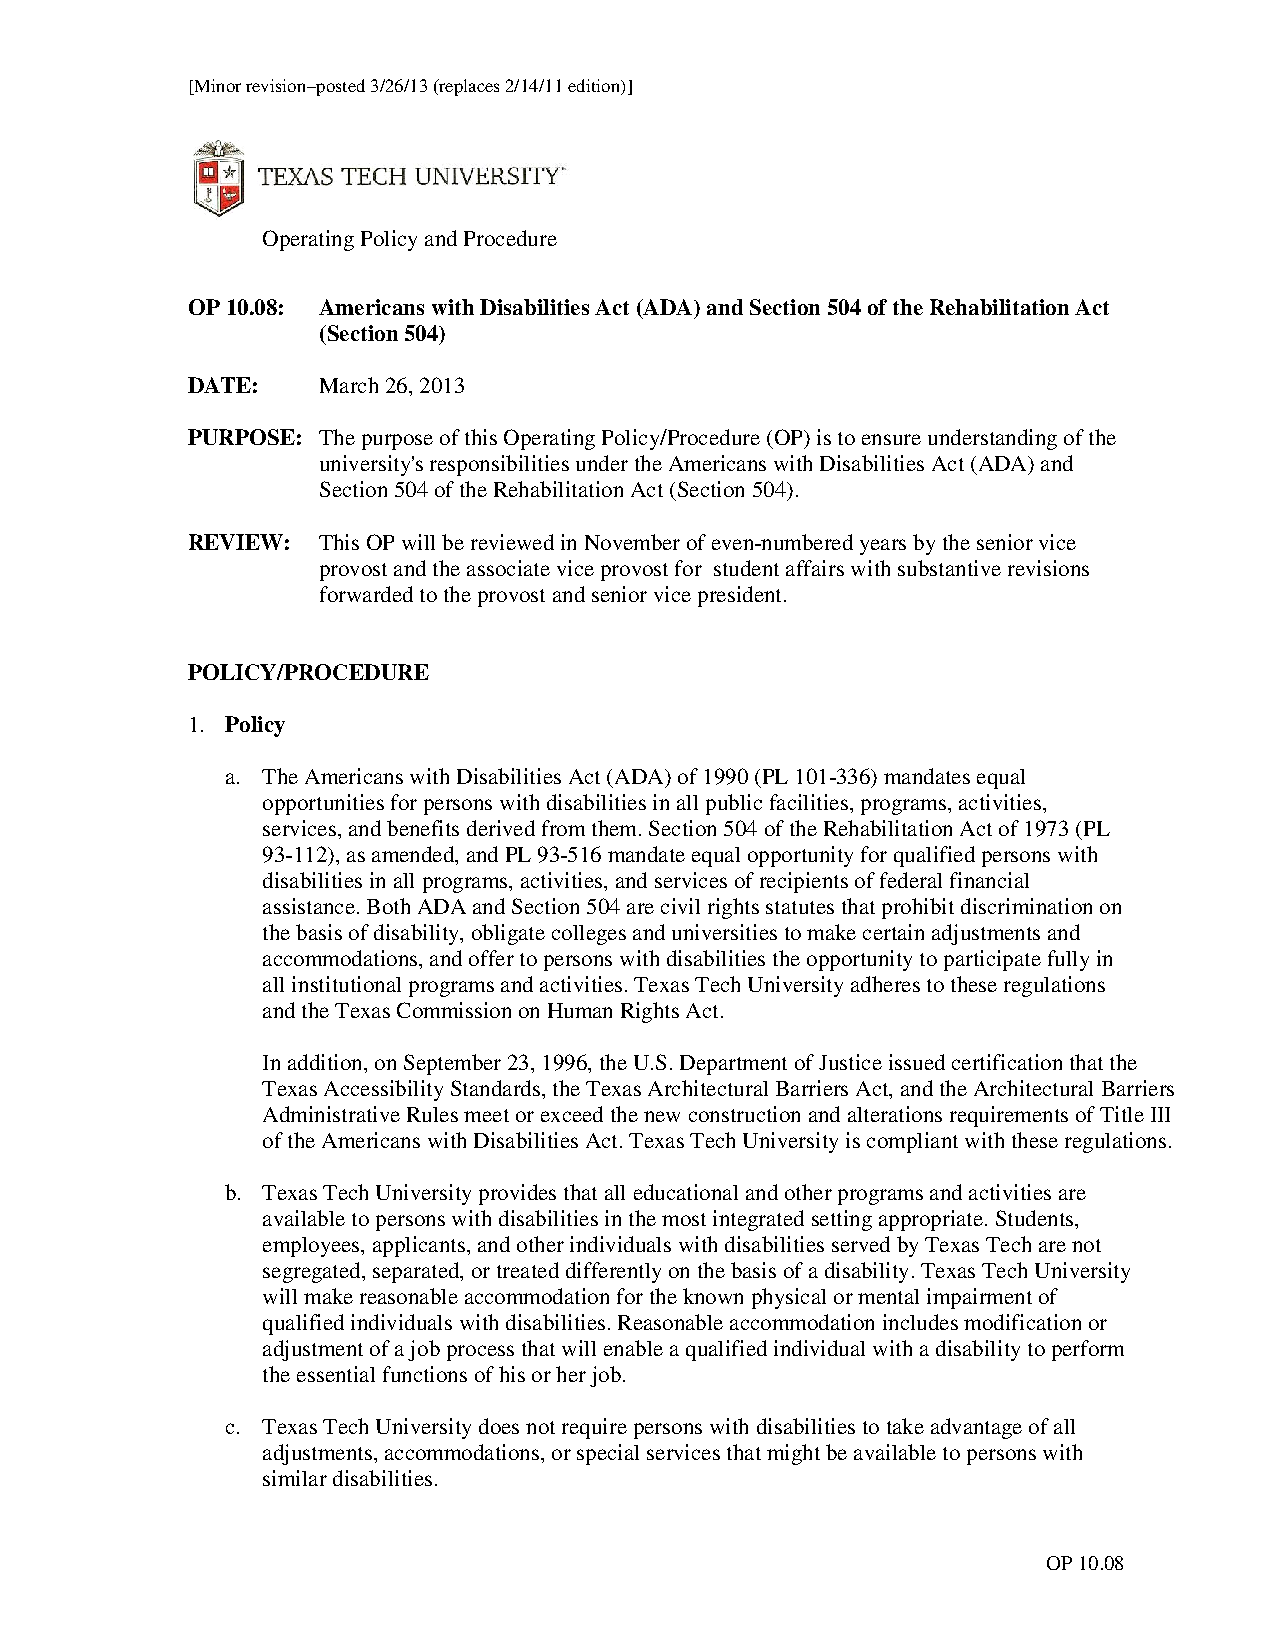
\includepdf[pages=-]{./OP10-08.pdf}

\section*{Required Syllabus Statements}
\url{https://www.depts.ttu.edu/tlpdc/RequiredSyllabusStatements.php}
\subsection*{ADA STATEMENT:}
Any student who, because of a disability, may require special arrangements in order to meet the course requirements should contact the instructor as soon as possible to make any necessary arrangements. Students should present appropriate verification from Student Disability Services during the instructor's office hours. Please note: instructors are not allowed to provide classroom accommodations to a student until appropriate verification from Student Disability Services has been provided. For additional information, please contact Student Disability Services in Weeks Hall or call 806-742-2405.

\subsection*{ACADEMIC INTEGRITY STATEMENT:}
Academic integrity is taking responsibility for one's own class and/or course work, being individually accountable, and demonstrating intellectual honesty and ethical behavior. Academic integrity is a personal choice to abide by the standards of intellectual honesty and responsibility. Because education is a shared effort to achieve learning through the exchange of ideas, students, faculty, and staff have the collective responsibility to build mutual trust and respect. Ethical behavior and independent thought are essential for the highest level of academic achievement, which then must be measured. Academic achievement includes scholarship, teaching, and learning, all of which are shared endeavors. Grades are a device used to quantify the successful accumulation of knowledge through learning. Adhering to the standards of academic integrity ensures grades are earned honestly. Academic integrity is the foundation upon which students, faculty, and staff build their educational and professional careers. [Texas Tech University (“University”) Quality Enhancement Plan, Academic Integrity Task Force, 2010].


\subsection*{RELIGIOUS HOLY DAY STATEMENT:}
"Religious holy day" means a holy day observed by a religion whose places of worship are exempt from property taxation under Texas Tax Code §11.20. A student who intends to observe a religious holy day should make that intention known in writing to the instructor prior to the absence. A student who is absent from classes for the observance of a religious holy day shall be allowed to take an examination or complete an assignment scheduled for that day within a reasonable time after the absence. A student who is excused under section 2 may not be penalized for the absence; however, the instructor may respond appropriately if the student fails to complete the assignment satisfactorily.

\subsection*{STATEMENT OF ACCOMMODATION FOR PREGNANT STUDENTS:}
To support the academic success of pregnant and parenting students and students with pregnancy related conditions, the University offers reasonable modifications based on the student's particular needs. Any student who is pregnant or parenting a child up to age 18 or has conditions related to pregnancy may contact Alex Faris, the Texas Tech University designated Pregnancy and Parenting Liaison, to discuss support available through the University. The Liaison can be reached by emailing alfaris@ttu.edu. Should a student communicate with the instructor that they are pregnant or have a pregnancy related condition or may need additional resources related to pregnancy or parenting, the instructor will communicate that student's information to the Title IX Coordinator, who will work with the student and others, as needed, to ensure equal access to the University's education program or activity. 

For more information regarding supportive measures, please contact pregnancy \& parenting liaison Alex Faris (alfaris@ttu.edu : 806.834.3420) or visit \url{https://www.depts.ttu.edu/titleix/PregnacnyandParenting/index.php}. 
You can also visit \url{https://www.depts.ttu.edu/titleix/PregnacnyandParenting/index.php} to submit a request to Alex Faris for assistance.

\section*{Recomended/Optional Syllabus Statements}
\url{https://www.depts.ttu.edu/tlpdc/RecommendedSyllabusStatements.php}

\subsection*{DISCRIMINATION, HARASSMENT, AND SEXUAL VIOLENCE STATEMENT:}

Texas Tech University is committed to providing and strengthening an educational, working, and living environment where students, faculty, staff, and visitors are free from gender and/or sex discrimination of any kind. Sexual assault, discrimination, harassment, and other Title IX violations are not tolerated by the University. Report any incidents to the Office for Student Rights \& Resolution, (806)-742-SAFE (7233) or file a report online at \url{titleix.ttu.edu/students}. Faculty and staff members at TTU are committed to connecting you to resources on campus. Some of these available resources are: 
\begin{itemize}
\item TTU Student Counseling Center, 806- 742-3674, \url{https://www.depts.ttu.edu/scc/}(Provides confidential support on campus.) 
\item TTU 24-hour Crisis Helpline, 806-742-5555, (Assists students who are experiencing a mental health or interpersonal violence crisis. If you call the helpline, you will speak with a mental health counselor.) 
\item Voice of Hope Lubbock Rape Crisis Center, 806-763-7273, \url{voiceofhopelubbock.org} (24-hour hotline that provides support for survivors of sexual violence.) 
\item The Risk, Intervention, Safety and Education (RISE) Office, 806-742-2110, \url{https://www.depts.ttu.edu/rise/} (Provides a range of resources and support options focused on prevention education and student wellness.) 
\item Texas Tech Police Department, 806-742-3931, \url{http://www.depts.ttu.edu/ttpd/} (To report criminal activity that occurs on or near Texas Tech campus.)
\end{itemize}
 
\subsection*{RECOVERY SERVICES STATEMENT:}

The Center for Students in Addiction Recovery offers students in recovery a nurturing and supportive community. The Center provides students in recovery with an abstinence-based program where students can flourish in recovery as they attain educational goals, including advanced degrees. The services provided through the CSAR increases the continuum of care for students in recovery, enhancing the quality of life for students in recovery at Texas Tech University. The CSAR supports students in recovery from alcohol, drugs, and behavioral addictions. By providing recovery support through relationships with staff, academic advising, scholarships / fellowships, recovery housing, study abroad opportunities, and more, students can flourish in recovery and in life.

 
\subsection*{CIVILITY IN THE CLASSROOM STATEMENT:}

Texas Tech University is a community of faculty, students, and staff that enjoys an expectation of cooperation, professionalism, and civility during the conduct of all forms of university business, including the conduct of student–student and student–faculty interactions in and out of the classroom. Further, the classroom is a setting in which an exchange of ideas and creative thinking should be encouraged and where intellectual growth and development are fostered. Students who disrupt this classroom mission by rude, sarcastic, threatening, abusive or obscene language and/or behavior will be subject to appropriate sanctions according to university policy. Likewise, faculty members are expected to maintain the highest standards of professionalism in all interactions with all constituents of the university (\url{www.depts.ttu.edu/ethics/matadorchallenge/ethicalprinciples.php}).

 
\subsection*{PLAGIARISM STATEMENT:}

Texas Tech University expects students to “understand the principles of academic integrity and abide by them in all class and/or course work at the University” (OP 34.12.5). Plagiarism is a form of academic misconduct that involves (1) the representation of words, ideas, illustrations, structure, computer code, other expression, or media of another as one's own and/or failing to properly cite direct, paraphrased, or summarized materials; or (2) self-plagiarism, which involves the submission of the same academic work more than once without the prior permission of the instructor and/or failure to correctly cite previous work written by the same student. This video, retrieved from the University of Kansas Libraries website, provides an example of a plagiarism definition as well as examples of plagiarism and how to avoid it. Please review Section B of the TTU Student Handbook for more information related to other forms of academic misconduct, and contact your instructor if you have questions about plagiarism or other academic concerns in your courses. To learn more about the importance of academic integrity and practical tips for avoiding plagiarism, explore the resources provided by the TTU Library and the School of Law.

 
\subsection*{STUDENT SUPPORT STATEMENT:}

The Office of Campus Access and Engagement works across Texas Tech University to foster, affirm, celebrate, engage, and strengthen all student communities. For more information about services, opportunities for participation, and ways in which Texas Tech can support your success in college, please contact (806) 742-7025.

 
\subsection*{STATEMENT ABOUT FOOD INSECURITY:}

Any student who faces challenges securing their food or housing and believes this may affect their performance in the course is urged to contact the Dean of Students for support. Furthermore, please notify the professor if you are comfortable in doing so. Raider Red's Food Pantry (located in Doak 117) supplies personal care items and a selection of nonperishable food to students. The Raider Relief Advocacy and Resource Center (RR- ARC) is a centralized hub of resources and support for students facing hardships with their basic needs. Through a comprehensive network of campus and community partnerships, we strive to alleviate the burden of financial, physical, and emotional hardships and promote the well-being and academic success of all students. Please fill out our form to get connected: \url{https://www.depts.ttu.edu/raiderrelief/}.

 
\subsection*{RISK ASSOCIATED WITH THE USE OF LIVESTOCK/HORSES STATEMENT:}

Working with livestock is inherently risky. Animals are capable of injuring people, especially when they are in the fight or flight mode in response to stress or unfamiliar situations. The instructor will work to provide students with the ability to manage horses or livestock with minimal stress, thus decreasing the risk of injury to people and animals. It is imperative that students follow instructions and communicate any discomfort with assigned activities. Please see link for additional information on animal-borne diseases: \url{https://www.depts.ttu.edu/iacuc/Zoonoses_Guidelines.php}

 
\subsection*{RISK ASSOCIATED WITH THE USE OF COMPANION ANIMALS STATEMENT:}

Working with companion animals can be inherently risky. Dogs and cats are capable of injuring people, especially when they are fearful or in unfamiliar situations. The instructor will work to provide students with the ability to handle dogs and cats with minimal stress, thus decreasing the risk of injury to people and animals. It is imperative that students follow instructions and communicate any discomfort with assigned activities. Please see link for additional information on animal-borne diseases: \url{https://www.depts.ttu.edu/iacuc/Zoonoses_Guidelines.php}

 
\subsection*{RISK ASSOCIATED WITH THE USE OF WILDLIFE STATEMENT:}

Working with wildlife is inherently risky. Some wildlife species are capable of injuring people and/or spreading zoonotic diseases. The instructor will work to provide students with the ability to handle wildlife species with minimal stress, thus decreasing the risk of injury to people and animals. It is imperative that students follow instructions and communicate any discomfort with assigned activities. Please see link for additional information on animal-borne diseases: \url{https://www.depts.ttu.edu/iacuc/Zoonoses_Guidelines.php}

\section*{AI Use Syllabus Statements:}
\url{https://www.depts.ttu.edu/tlpdc/AI_Resources/AI-Use-is-Encouraged.pdf}
\subsection*{AI Use is encouraged and allowed in your course:}
You may use generative artificial intelligence (AI) tools (such as ChatGPT) in this class, as doing so aligns with our course learning goals. Your use of AI tools must be properly documented and cited. You are responsible for ensuring the information you submit based on an AI query does not contain misinformation, unethical content, or violate intellectual property laws. Submission of AI-generated content as your own work is a violation of academic integrity and may result in referral to the Office of Student Conduct. Please contact your instructor if you have questions regarding this course policy.\footnote{AI responses are often incorrect; be sure the response makes sense, is correct, and grammatically edited.  AI responses must be disclosed in your work.}





\begin{thebibliography}{}

\bibitem[Chow and others(1988)]{CMM1988}
Chow, V.T., Maidment, D.R., Mays, L.W., 1988, Applied Hydrology: New York,
McGraw-Hill.

\bibitem[Dooge(1973)]{Dooge1973}
Dooge, J.C.I. 1973.  Linear Theory of Hydrologic Systems. ARS Technical Bulletin No. 1468.  US Department of Agriculture, Washington, D.C.

\bibitem[McCuen and others(2002)]{McCuen2002}
Richard H. McCuen, Peggy A. Johnson, Robert M. Ragan, 2002.  Highway Hydrology; Hydraulic Design Series Number 2, Second Edition.  
Federal Highway Administration, National Highway Institute, 4600 North Fairfax Drive, Suite 800, Arlington, Virginia 22203.  424p.

\bibitem[Gupta(2017)]{Gupta2017}
Gupta, R.S. 2017. Hydrology and Hydraulic Systems 4th ed. Waveland Press, Inc. ISBN 978-1-4786-3091-3 888p.

\bibitem[Cleveland(2024)]{Cleveland2024}
Cleveland, T. G. 2024. Engineering Hydrology Instructor's Notes and Selected Readings to accompany CE-3354, Department of Civil, Environmental, and Construction Engineering, Whitacre College of Engineering. \url{http://54.243.252.9/ce-3354-webroot/}

\end{thebibliography}

\end{document}  

\subsection*{{Knowledge, Skills, Abilities (KSA)}}
During this course the student will
\begin{enumerate}
\item Read, synthesize, and communicate ideas presented in current and historical technical literature.
\item Delineate watersheds from maps and determine common metrics (area, slope, main channel length) using digital planimetry.
\item Perform hydrologic computations using Excel, as needed\footnote{This task is principally to develop understanding of how the professional tools function.  Excel is a professional tool in its own right, but the skill level to use for engineering is beyond the scope of this class.}.
\item Perform hydrologic simulation using HEC-HMS (large-scale) and/or USEPA SWMM (small-scale).
\item Size and select engineering materials (pipes) for use in drainage engineering.
\item Prepare professional reports for the design of a stormwater management system.  

\end{enumerate}